\documentclass{TDP005mall}
\usepackage{graphicx}


\newcommand{\version}{Version 1.0}
\author{Elliot Johansson, \url{elljo130@student.liu.se}\\
  Lukas Freyland, \url{lukfr510@student.liu.se}\\
  Nadim Lakrouz, \url{nadla777@student.liu.se}}
\title{Designspecifikation}
\date{2022-11-25}
\rhead{Elliot Johansson\\
  Lukas Freyland\\
  Nadim Lakrouz}



\begin{document}
\projectpage
\section{Revisionshistorik}
\begin{table}[!h]
  \begin{tabularx}{\linewidth}{|l|X|l|}
    \hline
    Ver. & Revisionsbeskrivning & Datum \\\hline

    1.0 & Första utkast & 2022-11-25 \\\hline
  \end{tabularx}
\end{table}

\section{Player}

Syftet med Playerklassen är att representera den karaktär spelaren styr. Spelaren styr vilka formler playerkaraktären använder. Spelaren kommer inte förflytta sig på planen. Vissa formler kommer behöva riktas för att träffa fienderna medan andra inte behöver det.
Funktionen regenerate\_mana kommer sakta återställa manapoäng med sf:Clock.

\subsection{}

\begin{itemize}
\item int hp - privat variabel som tilldelas ett heltal. 
\item double mana - privat variabel som tilldelas ett flyttal. 
\item sf:Clock clock - sfml variabel för att hantera tiden.
\item int set\_hp() - ändrar privata variabeln hp.
\item int get\_hp() - hämtar privata variabeln hp.
\item int get\_mana() - hämtar privata variabeln mana.
\item void regenerate\_mana() - ökar privata variabeln mana över tid.
  
\end{itemize}


\section{Enemies}
''Enemies'' klassens syfte är att representera fienderna som i intervaller kommer förflytta sig mot spelaren på spelplanen. Enemies har en check\_collision funktion som anropas när fiender och spelare kolliderar.
\subsection{}

\begin{itemize}

%% \item double hp - privat variabel som tilldelas ett flyttal. 
%% \item double resistance - privat variabel som tilldelas ett flyttal.
%% \item void check\_collision() - kollar kollision med spelaren och magiska formler. 
%% \item int set\_hp() - ändrar privata variabeln hp.
%% \item int get\_hp() - hämtar privata variabeln hp.
%% \item int get\_resistance() - hämtar privata variabeln resistancce.
  %% \item void ai\_movement() - styr fiende rörelse.
\item float yValue - förvarar y position.
\item float xValue - förvarar x position.
\item float size - fövarar storlek på fiende.
\item double x\_movement - förvarar förflyttningen i x led.
\item CircleShape circle - förvarar cirkeln som representerar fienden.
\item Vector2f location - förvarar fiendens position.
\item Texture texture - förvarar fiendens textur.
\item void update() - ändrar fiendens position.
\item void render - ritar ut fienden.
\item CircleShape getCircle() - returnerar cirkeln som representerar fienden.
\item void setLocation() - bestämmer fiendens nästa position.
\item Vector2f getLocation() - returnerar fiendens position.
\item int getDistanceCircles() - returnerar avståndet mellan två fiender.
\item bool checkCollision() - returnerar true om två fiender överlappar.
\item double get\_x\_Movement() - returnerar hur mycket en fiende ska förflyttas i x led varje förflyttning.
  
\end{itemize}


\section{enemyHandler}

\begin{itemize}

\item vector<Enemy*> enemy\_container - vector av enemy pekare.
\item Time render\_time - förvarar frekvensen som fiender ska ritas ut med.
\item Time enemy\_create\_time - förvarar frekvensen som fiender skapas med.
\item Clock clock - skapar en klocka som räknar tiden.
  
\item void createNewEnemy() - skapar ny fiende och förvarar i vector av pekare.
\item vector<Enemy*> getEnemies() - returnerar vector av enemy pekare.
\item void rendering() - ritar ut varje fiende.
  
\end{itemize}


\section{Spells\_Handler}

\begin{itemize}

\item pair<string, int> mana\_per\_spell - lista med hur mycket mana varje magiska formel kostar. 
\item void handle\_input() - hanterar spelarens inmätning. 
\item void handle\_combination() - hanterar kombinationer av magiska     formler. 
\item void handle\_damage() - beräknar och hanterar damage. 
\item void control\_spell() - navigerar spells med hjälp av mus. 
  
\end{itemize}


\section{}

\begin{itemize}
  
\item
  
\end{itemize}


\section{Engine}

\begin{itemize}
\item int current\_state - förvarar vilket state spelet befinner sig i.
\item RenderWindow window - fönstret som allt renderas i.
\item map<int, unique\_ptr> states - förvarar de olika statesen.

\item Engine() - konstruktor.
\item int run() - kör spelet.
\end{itemize}


\section{Base\_State}

\begin{itemize}
  
\item unsigned int curr\_state - nuvarande state.
\item virtual ~Base\_State() - destruktor.
\item virtual void update() - uppdatera state logiken.
\item virtual void render() - renderar det som ska visas.
\item virtual int get\_current\_state() - returnera nuvarande state.
\item virtual int get\_next\_state() - returnerar nästa state.
\item 
\item
\item
\item
  
\end{itemize}


\section{utility}

\begin{itemize}
  
\item bool debounce() - kollar om knapp är nedtryckt.
\item debug\_print() - skriver ut debug text.
  
  
\end{itemize}


\section{Button\_Manager}

\begin{itemize}
  
\item Button\_Manager() - konstruktor
\item void update() - 
\item void render() - 
  
\end{itemize}





\section{Diagram}
\begin{center}
  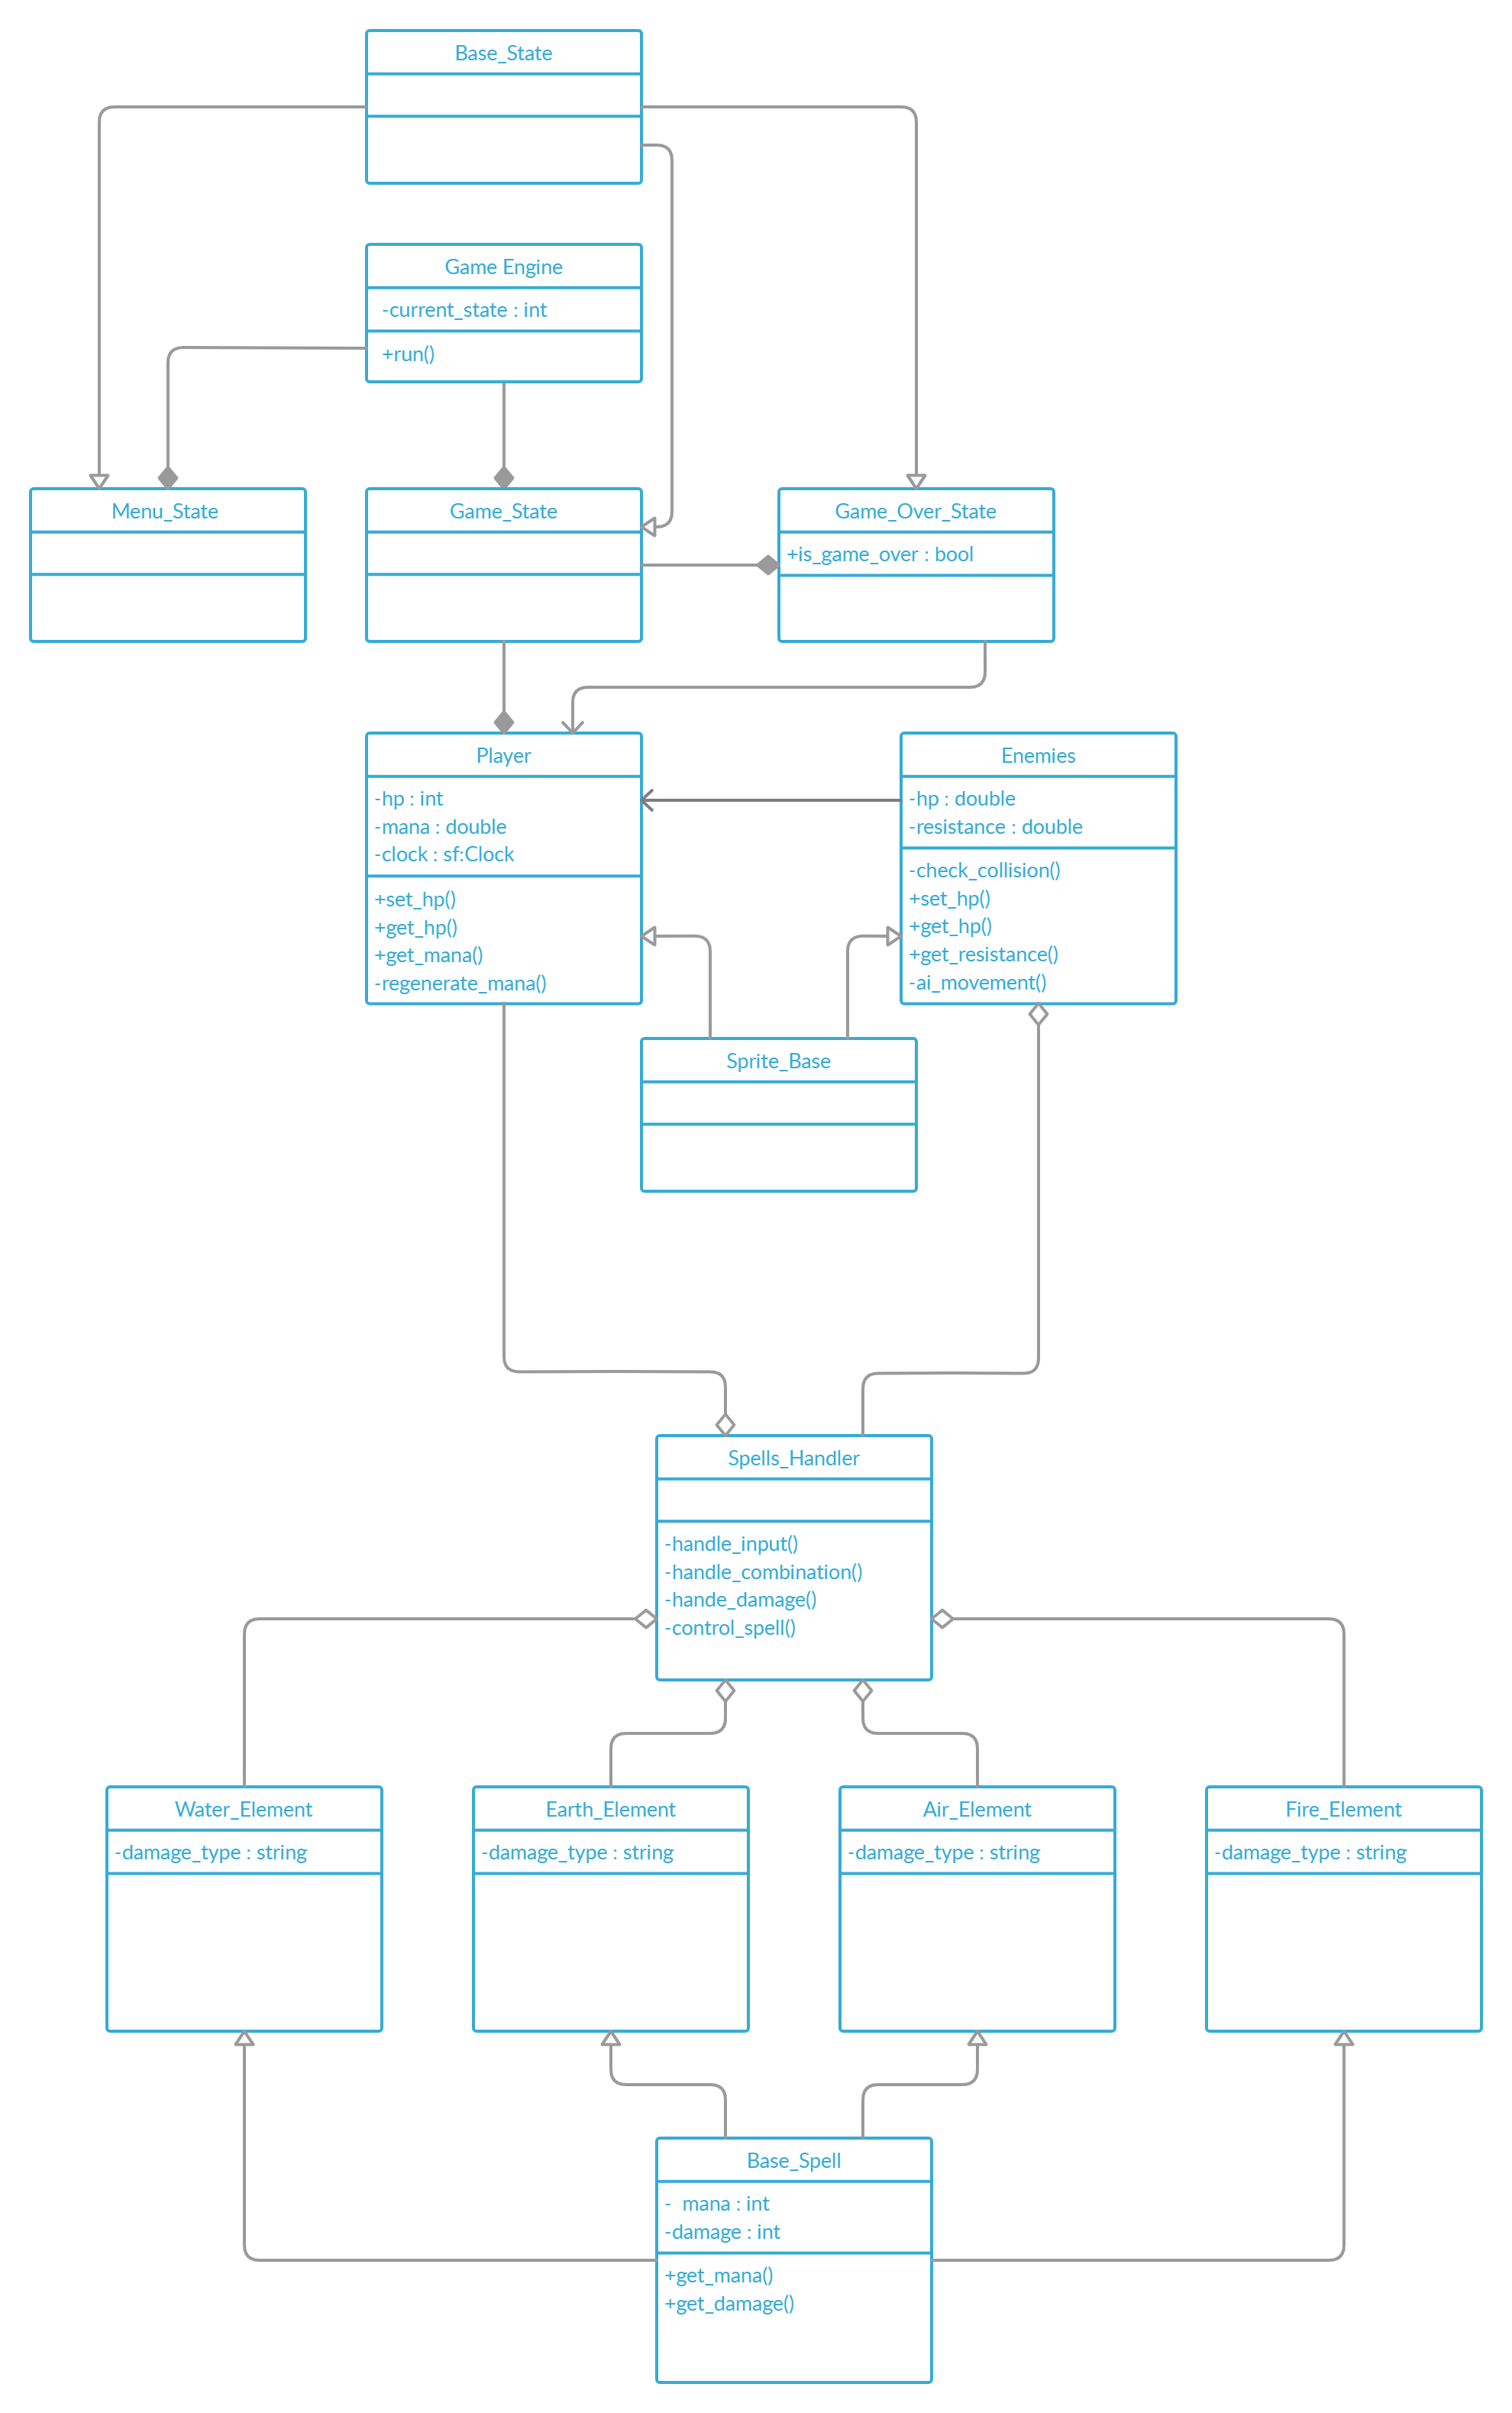
\includegraphics[scale=0.18]{uml_diagram.jpg}
\end{center}
\end{document}
